\documentclass[../main.tex]{subfiles}
\begin{document}
\setchapterimage[6.5cm]{Images/boh.jpg}
\setchapterpreamble[u]{\margintoc}
\chapter[Lectures by Prof. Contino]{Lectures by Prof. Contino\footnotemark[0]}
\labch{rc}
\section{Accidental Symmetries of the Standard Model}
The \textbf{gauge group} of the Standard Model is given by\\ G=SU$(3)_{\text{C}}\times$SU$(2)_{\text{EW}}\times$U$(1)_{\text{Y}}$ and when we write the Lagrangian we know that the rules of the game are that we should write every single term allowed by this symmetry and by Lorentz invariance. Then we write all the terms and we may discover that, in addition to the invariance under this symmetry and under Lorentz, there is also invariance under some global symmetry group which comes for free because we did not impose it. Of course we could have imposed the requirement of invariance under some global group by hand, i.e. for phenomenological reasons. But in the SM we do not do it, we do not require invariance under any global symmetry group. The only thing we do is to impose invariance under G and under Lorentz, these are the only two requirements.\\
Now the question is: \textit{is this Lagrangian invariant under some global symmetry?}\marginnote{We do not write the Lagrangian again, we did it in \refch{intro}} Obviously, the answer is \textbf{yes}. There are two discrete symmetries, parity and charge conjugation which are then violated, but it turns out there are actually \textbf{continuous symmetries} which are invariant transformations of the Lagrangian. How can we see these symmetries? We try to transform fields in a way which has to respect gauge invariance. This means that if we have a certain representation under the gauge group we have several fields transforming under this representation and it is possible to mix them among themselves and that could be a symmetry transformations. Do we have replicas? Yes, we have three families. It is possible to transform fields by mixing these families and this is something which respects Lorentz and gauge invariance. That is the global symmetry that we might have, whether we have it or not depends on the Lagrangian, more precisely whether such transformations leave the Lagrangian invariant or not.\\ 
The kinetic term for the $q_L$ for example can be written in such a way that it is diagonal in flavour:
\[
\overline{q}_L^ii\slashed{D}\delta^{ij}q^j
\]
which is symmetric under $\text{U}(3)$. However, there are additional terms like the Yukawa coupling which breaks this symmetry. It turns out that there is some symmetry leftover. If we restrict it to the quark sector, we have a $[\text{U}(3)]^3$ symmetry:
\[
\pazocal{L}_{\text{kin}}=\overline{q}_L^ii\slashed{D}\delta^{ij}q_L^j+\overline{u}_R^ii\slashed{D}\delta^{ij}u_R^j+\overline{d}_R^ii\slashed{D}\delta^{ij}d_R^j
\]
If we move to the basis where the Yukawa matrices are diagonal we have:
% Each quark has \textbf{baryon number} $B(q)=+1/3$ which results for protons and neutrons in $B(p)=B(n)=1$ being $p=uud$ and $n=udd$. Moving to the basis where the Yukawa term is diagonal we have:
\[
\frac{1}{\sqrt{2}}\overline{u}_L^i\delta^{ij}(v+h)u_R^j+\frac{1}{\sqrt{2}}\overline{d}_L^i\delta^{ij}(v+h)d_R^j+\text{h.c.}+g\overline{u}_L^iV^{ij}W_\mu^-\gamma^\mu d_L^j+\text{h.c.}\marginnote{We are not including leptons just for simplicity.}
\]
There are U(1) factors which are unbroken and in particular for the quarks there is a U(1) \textbf{baryon number} which is unbroken by the Yukawa terms. How can we see it? By diagonalizing the Yukawa matrices, we see that the Yukawa terms couple quarks with the same charge and if we do a transformation under which all the quarks go like:
\[
q\to e^{i\alpha/3}q
\]
this leaves the Yukawa terms, and in general the Lagrangian, invariant. If we do transformations of $[\text{U}(3)]^3$ these terms are not invariant but if we do transformations like the one above which is a subgroup of the larger symmetry,  U$(1)_{\text{B}}\subset[\text{U}(3)]^3$, all the quarks have the same charge, i.e. baryon number $B(q)=+1/3$.\marginnote{This +1/3 is arbitrary, the important thing is that it is the same for all the quarks. It is taken to be +1/3 because in this way protons and neutrons for example have $B(p)=B(n)=+1$.}\\
This is the only leftover global symmetry which remains in this Lagrangian, it is not broken by any term and the best way to see it is by going to the basis in which the Yukawa couplings are diagonal.

If we try do to the same with leptons there is a complication and a simplification. The simplification is due to the fact that we do not have a right-handed neutrino because up to now there is no experimental evidence that we need it but the complication is that we do observe oscillations between different flavours of neutrinos. This is possible only if the neutrinos have a mass and in the Lagrangian that we wrote neutrinos \textit{do not} have a mass, there is no term which gives the mass of the neutrinos.\\
How do we fix this problem? There are two possibilities: we \textit{either} extend the model by adding a new light degree of freedom, the right-handed neutrino $\nu_R$, \textit{or} since the SM is an EFT then we can consider higher dimension operators. We only wrote dimension 4 operators which do not give a mass to the neutrinos but moving to higher dimensions there are new operators which do give a mass to the neutrinos.\\
The next dimensionality is $D=5$ and the only operator we have is the \textbf{Weinberg operator}. How can we write a dimension 5 operator? The only possibility is to put two fermions and two scalars but it also has to be gauge and Lorentz invariant. Since we know that the hypercharge for a doublet of leptons is $-1/2$ and for the Higgs is $+1/2$, the following combination is neutral under the hypercharge:
\[
(l_L^{\alpha,i} H)(l_L^{\beta,j} H)\epsilon_{\alpha\beta}
\]
where the $\epsilon$ tensor is required to make this object a singlet, $\alpha$ and $\beta$ are Lorentz indices and $i,j$ are SU$(2)_{\text{EW}}$ indices. The thing we need to check is whether the exchange of these two leptons imply the right symmetry\marginnote{Another possible way to see it is by using the functional integral where the two fermionic fields are Grassmann variables.}. The fermionic nature gives us a $(-)$ sign under exchange and the $\epsilon$ tensor gives another $(-)$ sign so there is an overall $(+)$. Contracting this with another $\epsilon$ tensor gives a final $(-)$ sign which is bad so this possibility is not allowed. \raisebox{-\mydepth}{{
\includegraphics[height=1.1\baselineskip]{Images/sadsmile.jpg}}}\\
What we can do is the following:
\[
O_{\text{Weinberg}}:=\frac{1}{M}\epsilon^{ik}(l_L^{\alpha,i}H^k)R(l_L^{\beta,j}H^s)\epsilon_{\alpha\beta}\epsilon_{js}
\]
This is the Weinberg operator which is an invariant. If we go to the unitary gauge, $H$ can be written as $H=\frac{1}{\sqrt{2}}\begin{pmatrix}0\\v+h\end{pmatrix}$ so, at lowest order, the operator becomes:
\[
O_{\text{Weinberg}}=\nu_L^{\alpha,a}\nu_L^{\beta,b}v^2\frac{R^{ab}_{\text{Weinberg}}}{2M}\epsilon_{\alpha\beta}+\cdots
\]
where $a$ and $b$ are flavour indices. This is the mass term for neutrinos, $1/M$ is a coefficient required for dimensionality reasons. $R$ is a matrix which scales like a coupling squared because there are four fields.\\ 
This tells us that if the extension of the SM is in the form of heavy new physics, it is possible to interpret this operator as arising from some new particles which are integrated out. With this supposed new heavy physics, it turns out that we do see effects of this higher dimensional operators through observing the neutrino masses.\\
The other possibility is to add the right-handed neutrino which is light and that is not captured by this story. This argument is okay if there is heavy new physics, in other words if the light right-handed neutrino cannot be integrated out. Of course there is the mixed possibility that the new physics which gives rise to this operator is a heavy right-handed neutrino.\\
This goes under the name of \textbf{seesaw mechanism}.\marginnote{
\includegraphics[]{Images/seesaw.png}\\From \href{https://www.symmetrymagazine.org/article/neutrinos-on-a-seesaw}{Symmetry Magazine}, a funny representation of the seesaw mechanism.} The right-handed neutrino $\nu_R$ is neutral under G, it is a singlet both under SU$(3)_{\text{C}}$ and SU$(2)_{\text{EW}}$ and it has zero hypercharge. This should ring a bell, if we have something which is a Weyl fermion and completely neutral it is possible to write a \textbf{Majorana mass term}:
\[
\nu_R^{\alpha,a}M^{ab}\nu_R^{\beta,b}\epsilon_{\alpha\beta}
\]
where $M^{ab}$ has to be symmetric.\\
Majorana particles have two polarizations but particle and anti-particle are identical. This is the main difference between a Weyl fermion and a Majorana fermion, strictly speaking we should talk about Weyl fermions only for massless fermions. Weyl fermions have only one polarization, which corresponds to helicity since it is massless, and then particle and anti-particle, hence two degrees of freedom. When imposing the condition that allows us to write the Majorana mass term, then we are identifying particle with anti-particle which means that there will be two degrees of freedom interpreted as particle with polarization $+1/2$ and particle with polarization $-1/2$. The point is that this mass term can be interpreted as an interaction between two $\nu_R$.\\
What is the value of $M^{ab}$? Naively, we could interpret our theory as an EFT, not including $\nu_R$ so it will be valid up to some cut-off scale above which there will be new physics. What are the coefficients in front of the terms in the Lagrangian? The mass term has dimension 3, so these terms will have coefficients of dimension 1. Remember that there is another term which has dimension smaller than 4, the Higgs term $H^\dagger H$ which has a coefficient $\mu^2$ of dimension 2. These are the only two relevant operators\marginnote{Relevant in a sense that they are the only operators with dimension strictly smaller than 4.}. If we set these coefficients to values much smaller than the scale of new physics we want to see whether radiative corrections will give a noticeable contributions to them.\\
In other words: \textit{if we set these two terms to be much smaller than the cut-off scale will radiative corrections destroy the assumptions we made?} The answer is \textbf{yes}, there will be huge radiative corrections and the idea of setting $\mu$ to a small value is hopeless.\\
This problem is known as the \textbf{hierarchy problem} which can be summarized as follows: we need $\mu$ of order $v$, $v$ is of order of the electroweak scale 246 GeV so we say \textit{okay, we write $\mu$ and say it is of order 246 GeV}. But then we go to one-loop level to include radiative corrections of this form:\\
\begin{figure}[h]
    \centering
    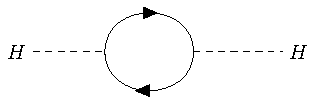
\includegraphics[width=0.6\textwidth]{Images/higgscorrections.pdf}
    \caption*{}
    \labfig{higgscorrections}
\end{figure}\\
Doing the calculations, we see that this diagram is quadratically divergent and it goes like $\Lambda^2\frac{y_\Psi^2}{16\pi^2}$. If we assume that $\Lambda$ is of order of the Planck scale, the suppression coming from the Yukawa coupling is small\marginnote{(Not so) technical term: \textit{this suppression is peanuts}} so if we set $\mu$ to be of order 246 GeV at tree-level, at one-loop it will become of order Planck. There is no hope to get a light Higgs.\\
This problem requires a precise cancellation between the radiative corrections and the tree-level term.\\
The $\nu_R$ is a fermionic field with chiral invariance associated broken by the mass term proportional to the one-loop corrections, so if the mass is light the corrections will be small. This is called \textbf{technical naturalness}. There is no danger in saying that this mass is much smaller than the cut-off scale so it will remain small even after radiative corrections are turned on. If this mass is heavy then we will have the seesaw mechanism: there is a heavy state that integrated out gives us very light state, because the mass of $\nu_L$ is suppressed. This is why it is called seesaw. However, we can also say that the mass is small, much smaller than the Planck scale, in which case this $\nu_R$ is an addition to the SM, it is not heavy new physics but rather light new physics.\\
We said there is an accidental U$(1)_{\text{B}}$ symmetry under which leptons do not transform. Is there an accidental symmetry regarding the lepton sector? Without $\nu_R$, the Yukawa term has the following form:
\[
\overline{l}_L^iY_l^{ij}He_R^j
\]
We can transform the doublet and the singlet with two unitary transformations and diagonalize $Y$ without touching the kinetic terms. Without inserting the additional structure for the mass of the neutrinos we do not have any counterpart of the CKM matrix, at this level there is no flavour mixing. We can then go to a basis in which $Y$ is diagonal and at this point then we can change the phases of the three different families independently. There is not one \textbf{lepton number} but there are three: $L_e, L_\mu$ and $L_\tau$. Under $L_e$, both the electron and the electronic neutrino transform with the same charge which is equal to 1 and the others do not transform. Under $L_\mu$ only the muon and the muonic neutrino transform with the same charge while the others do not transform and the same applies for $L_\tau$. It is possible to transform the fermion fields with different phases and this will keep every single term in the Lagrangian invariant. This accidental symmetry is a product of U$(1)_{\text{B}}$ and [U$(1)]^3$.\\
At least at the classical level, these are the exact global symmetries which emerge. Why are they called \textit{accidental}? Because they come as an accident at low energy, in the sense that the UV physics might not have them. In fact, if we write higher dimensional terms, e.g. $O_{\text{Weinberg}}$, we notice that they violate lepton number. If we say that the new physics has this symmetry then such a term is not allowed. But we are not imposing this symmetry by hand, we are just looking at low-energy and see which symmetries come out. This is the power of accidental symmetries: even if the UV theory is not invariant under that symmetry, at low-energy it emerges as an accident, it comes for free. They emerge because the theory is an EFT and because there is a large gap between the scale at which we do the experiments and the UV scale, which is much higher. Higher dimensional operators contribute to the experiments with the inverse power of the cut-off scale, they all violate these symmetries but their effects will be largely suppressed.\\
These symmetries are not truly \textit{exact} symmetries, they are exact only at $D=4$ but if we consider the theory as a whole they are \textit{approximate}. Accidental symmetries are important because they might be the only global symmetries that are allowed in nature because of gravity. This is an important issue when we try to include dark matter in our theory because as far as we can tell is not coming from the SM so we have the extend the theory. Where does the stability of DM come from? People would say \textit{okay, we introduce a global symmetry and make it stable}. Well, there is a problem. One possible way of arguing is that if such global symmetry exist, it is accidental.
\section{Fujikawa Approach to Anomalies}
A more direct connection between the anomaly and the violation of a symmetry uses the \textbf{path integral}. The idea, due to Fujikawa, is that anomalies arise when there are symmetries of the action that are not symmetries of the functional measure in the path integral. 
\[
Z[J]=\int\pazocal{D}\phi\exp{iS[\phi]+i\int d^4xJ(x)\phi(x)} 
\]
If the symmetry is anomalous, then the measure $\pazocal{D}\phi$ is not invariant. Consider now a fermionic field $\Psi(x)$ which transforms as:
\[
\Psi(x)\to e^{i\alpha^aT^a}\Psi(x)
\]
and assume that $\delta S=0$ for constant $\alpha^a$. For a local transformation, i.e. $\alpha^a=\alpha^a(x)$, we then have:
\[
\delta S=\int d^4x\partial_\mu\alpha^a(x)J^{\mu,a}(x)
\]
The functional integral has to be invariant under the following change of variables:
\[
d\Psi d\overline{\Psi}\to\exp{i\int d^4x\alpha^a(x)\pazocal{A}^a(x)}d\Psi d\overline{\Psi}
\]
where $\pazocal{A}^a(x)$ is the anomaly, given by:
\[
\pazocal{A}^a(x)=\frac{1}{16\pi^2}D^{abc}F_{\mu\nu}^b\Tilde{F}^{\mu\nu,c} \quad \left\{\begin{aligned}
&D^{abc}=\frac{1}{2}\Tr{T^a\{T^b,T^c\}}\\
&\Tilde{F}^{\mu\nu,c}=\frac{1}{2}\epsilon^{\mu\nu\rho\sigma}F_{\rho\sigma}^a
\end{aligned}\right.
\]
Therefore, we write:
\[
i\int d^4xd\Psi d\overline{\Psi}e^{iS}[\partial_\mu\alpha^aJ^{\mu,a}+\alpha^a\pazocal{A}^a]=0
\]
from which it follows:
\[
\int d\Psi d\overline{\Psi}e^{iS}\partial_\mu J^{\mu,a}=\pazocal{A}^a\int d\Psi d\overline{\Psi}e^{iS}
\]
To simplify the notation, it is possible to define:
\[
\Braket{O}_{A_\mu}:=\frac{\int d\Psi d\overline{\Psi}O(x)e^{iS}}{\int d\Psi d\overline{\Psi}e^{iS}}
\]
and the previous identity becomes:
\[
\Braket{\partial_\mu J^{\mu,a}}_{A_\mu}=\pazocal{A}^a=\frac{1}{16\pi^2}D^{abc}F_{\mu\nu}^b\Tilde{F}^{\mu\nu,c}
\]
Anomalies come from the fact that we cannot exhibit a regulator which respects global symmetry and gauge invariance, global symmetry gets broken. \marginnote{e.g. dimensional regularization breaks axial symmetry.} $D^{abc}$ automatically vanishes when:
\begin{enumerate}
    \item fields are in vector-like representations of the entire symmetry group, $\Psi_L$ in a representation $r$ and $\Psi_R$ in the same $r$.
    \[
    \Psi_R\to U\Psi_R\Rightarrow\Psi_R^C=U^*\Psi_R^C \quad U=\exp{i\alpha^aT^a}
    \]
    The generators can be written as $T^a=\text{diag}(t_L^a, -t_R^{aT})$ but in a vector-like representation we know that $t_L=t_R$:
    \begin{align*}
    D^{abc}&=\frac{1}{2}\Tr{t_L^a\{t_L^b,t_L^c\}}-\frac{1}{2}\Tr{(t_R^a)^T\{(t_R^b)^T,(t_R^c)^T\}}\\
    &=\frac{1}{2}\Tr{t_L^a\{t_L^b,t_L^c\}}-\frac{1}{2}\Tr{t_R^a\{t_R^b,t_R^c\}}=0
    \end{align*}
    This tells us that QCD is anomaly free, [SU$(3)_{\text{C}}]^3=0$ because it is vector-like.
    \item fields are in (pseudo-) real representations.\\
    This means that given a matrix $U$ such that $U^*=SUS^{-1}$, if the representation $r$ transforms under $U$ then $r$ is pseudo-real. If $T^a$ are purely imaginary then $r$ is real, the fundamental of SU(2) is a real representation: $(T^a)^T=-ST^aS^{-1}$. It then follows that:
    \begin{align*}
    D^{abc}&=\frac{1}{2}\Tr{T^a\{T^b,T^c\}}=\frac{1}{2}\Tr{(T^a)^T\{(T^b)^T,(T^c)^T\}}(-1)^3\\
    &=-D^{abc}\Rightarrow D^{abc}=0
    \end{align*}
\end{enumerate}
Groups with only real or pseudo-real representations are SO$(2n+1)$, SO$(2n)$ for $n\ge2$ and Sp$(2n)$ for $n\ge3$. Moreover, groups with complex representations but vanishing anomalies are SO$(4n+2)$ except for SO(2)=U(1) and SO(6)=SU(4).\\
Given this discussion about anomalies, we ask ourselves: \textit{is baryon number a good symmetry?} We can compute it:
\[
\left\{
\begin{aligned}
&q_L=\Box_{1/3}\,\text{of SU$(3)_{\text{C}}\times$U$(1)_{\text{B}}$} &&q_L=\begin{pmatrix}u_L\\d_L\end{pmatrix}\to q_L=\overbrace{(\Box,1/3)}^{r}\\
&q_R=\Box_{1/3}\,\text{of SU$(3)_{\text{C}}\times$U$(1)_{\text{B}}$} &&q_R=u_r,d_R\to q_R^c=\overbrace{(\overline{\Box},1/3)}^{\overline{r}}
\end{aligned}
\right.
\]
There is no anomaly of baryon number under SU$(3)_{\text{C}}$. How about under SU$(2)_{\text{EW}}$?
\[
D^{Bbc}=\frac{1}{2}\Tr{B}_{\text{weak doublets}}\Tr{\{T^b,T^c\}}=\frac{1}{2}\underset{\mathclap{\tikz \node {$\uparrow$} node [below=1ex] {\footnotesize  charge};}}{\frac{1}{3}}\cdot\overset{\mathclap{\tikz \node {$\downarrow$} node [above=1ex] {\footnotesize  colour};}}{3}N_f\delta^{bc}=N_f\frac{\delta^{bc}}{2}\marginnote{In the weak doublets, only $q_L$ contributes and it is factored out because it acts on a different space.}
\]
With the same strategy, we can compute the anomaly content under U$(1)_{\text{Y}}$:
\begin{align*}
D^{Byy}&=\frac{1}{2}\Tr{B}_{\text{quarks}}\Tr{\{Y,Y\}}\xleftarrow[]{}=2Y^2\\
&=N_f\left[\frac{1}{3}\cdot3\cdot2\left(\frac{1}{6}\right)^2+\left(-\frac{1}{3}\right)^2\cdot3\left(-\frac{2}{3}\right)^2+\left(-\frac{1}{3}\right)\cdot3\left(\frac{1}{3}\right)^2\right]\\
&=N_f\left[\frac{1}{2}\cdot\frac{1}{9}-\frac{4}{9}-\frac{1}{9}\right]=\frac{N_f}{9}\left(\frac{1}{2}-5\right)=-\frac{N_f}{2}
\end{align*}
This results in:
\[
\Braket{\partial_\mu J^\mu_B}=\frac{1}{16\pi^2}\frac{N_f}{2}[W_{\mu\nu}^i\Tilde{W}^{\mu\nu,i}-B_{\mu\nu}\Tilde{B}^{\mu\nu}]
\]
which is not a symmetry. At the classical level, there is a symmetry given by the product of baryon number and the three lepton numbers while at the quantum level instead we have:
\[
\text{U}(1)_{\text{B$-$L}}\times\text{U}(1)_{L_e-L_\mu}\times\text{U}(1)_{L_e-L_\tau}
\]
which is an accidental symmetry of the SM. In particular, B$-$L is anomalous and this is important if we want to extend the SM because it is not possible to gauge it.
% Suppose now that B$-$L is promoted to a gauge symmetry, what we need to check is [U$(1)_{\text{B$-$L}}]^3$ which is different from 0 in the SM but equal to 0 when we add $\nu_R$.
\section{SU(5) Grand Unification Theory}\marginnote[-1cm]{From \cite{CL}, Chapter 14.}
Elementary particle interactions are correctly described by the gauge group SU$(3)\times$SU$(2)\times$U$(1)$ down to distances as small as $10^{-16}$\,cm: QCD is the strong interaction theory and the Glashow-Weinberg-Salam model provides the theory of weak and electromagnetic interaction. It is desirable to have a more unified theory which can combine all three of these interactions as components of a single force, a theory with only one gauge coupling.\\
Georgi and Glashow showed that for the Standard Model the simplest unification gauge group of colour and flavour is SU(5) but because of the large differences in coupling strengths of strong and electroweak interactions, this unification would not become apparent until the energy scale of $10^{14}$ \,GeV, i.e. a distance of $10^{-28}$\,cm.\\
A general representation under an SU(5) transformation may be expressed as:
\[
\Psi^{ij\cdots}_{kl\cdots}\to U^i_mU^j_nU^s_kU^t_l\cdots\Psi^{mn\cdots}_{st\cdots}
\]
where all the indices run from 1 to 5 and:
\[
U^i_m=\exp{i\alpha^a\frac{\lambda^a}{2}}^i_m
\]
is a $5\times5$ unitary matrix. $\lambda^a$ with $a=0,1,\cdots,23$ is a set of 24 $5\times5$ generalized Gell-Mann matrices which are hermitian and traceless with normalization given by $\Tr{\lambda^a,\lambda^b}=2\delta^{ab}$. To obtain the SU$(3)\times$SU$(2)$ content of a representation we identify the first three of the SU(5) indices as the colour indices and the remaining two as SU$(2)_{\text{L}}$ indices:
\[
i=(\alpha,r) \quad \alpha=1,2,3 \quad r=4,5
\]
One family of fermions can be accommodated in an SU(5) reducible representation of $\overline{5}+10$:
\[
\overline{5}:\left(\begin{array}{c}
d_1^c\\d_2^c\\d_3^c\\l=\begin{pmatrix}\nu\\e
\end{pmatrix}
\end{array}\right) \quad
10: \left(\begin{array}{ccc:cc}
0 & u_3^c & -u_2^c & u_1 & d_1\\
-u_3^c & 0 & u_1^c & u_2 & d_2\\
u_2^c & -u_1^c & 0 & u_3 & d_3\\
\hdashline
-u_1 & -u_2 & -u_3 & 0 & e^+\\
-d_1 & -d_2 & -d_3 & -e^+ & 0
\end{array}\right)
\]
One consequence of the SU(5) scheme is an explanation for the experimentally observed charge quantization. This is because the eigenvalues of the generators of a simple non-abelian group are discrete while those corresponding to the abelian U(1) group are continuous.\marginnote{e.g. in the SO(3) group of rotations, the eigenvalues of the third component of the angular momentum can take only integer or half-integer values while in the U(1) symmetry of translation invariance in time there is no restriction on the eigenvalues of the corresponding generators.} Therefore in the SU(5) theory, since the electric charge $Q$ is one of the generators, its eigenvalues are discrete and hence quantized. The electric charge is an additive quantum number, so $Q$ must be some linear combination of the diagonal generators in SU(5). We then have:
\[
Q=T_3+\frac{1}{2}Y=T_3+cT_0
\]
where $T_3$ and $T_0$ are the diagonal generators belonging to the SU(2) and U(1) subgroups respectively.
\[
T_3=\frac{\lambda_3}{2}=\mqty(\dmat{0,0,0,\frac{1}{2},-\frac{1}{2}}) \quad T_0=\frac{\lambda_0}{2}=\frac{1}{\sqrt{15}}\mqty(\dmat{1,1,1,-\frac{3}{2},-\frac{3}{2}})
\]
The coefficient $c$ can be obtained by comparing the values of $T_0$ provided above and the hypercharge of the particles in the $\overline{5}$, giving us:
\[
c=-\sqrt{\frac{5}{3}}
\]
To check this result, we note that for the fundamental representation, combining all our knowledge discussed here we get:
\[
Q=\mqty(\dmat{-\frac{1}{3},-\frac{1}{3},-\frac{1}{3},1,0}):=Q_i\delta_{ij}
\]
and it follows that the fundamental conjugate representation $\overline{5}$ has $Q=-Q_i\delta-{ij}$. The most interesting aspect of charge quantization is the relation between colour SU(3) and charge. The traceless condition for the charge operator requires, for three colours:
\[
3Q_d+Q_{e^+}=0
\]
Quarks carry one third of the lepton charge because they have three colours. SU(5) then provides a rational basis for understanding particle charges.\\
The SU(5) adjoint representation has dimension $5^2-1=24$ and the following SU$(3)\times$SU$(2)$ decomposition:
\[
24=(8,1)+(1,3)+(1,1)+(3,2)+(\overline{3},2)
\]
$A_\beta^\alpha$ (8,1) are the SU(3) gluons $G_\beta^\alpha$, $A_s^r$ (1,3) are the three SU(2) vector fields $W$ and (1,1), given by a linear combination of $A_\alpha^\alpha$ and $A_r^r$ is the U(1) $B$-field. The remaining 12 fields have both SU(3) and SU(2) indices and they are denoted as $X,Y$ gauge bosons. These vector particles carry fractional charge:
\[
Q_X=-\frac{4}{3} \quad Q_Y=-\frac{1}{3}
\]
All the SU(5) gauge bosons can be put in a $5\times5$ matrix $A$ of the form:
\[
A=\frac{1}{2}\sum_{a=0}^{23}A^a\lambda^a
\]
\subsection{Proton Decay}
One prominent feature of the Grand Unification Theory is the non conservation of the baryon number. In the SM, baryon and lepton number are accidental, while the combination $B+L$ is anomalous: there is no proton decay mediated by anomalies.  The SU(5) model has this property and the leading effective Lagrangian for proton decay arises from a set of tree-level $X$ boson exchange diagrams. $X$ bosons couple to two-fermion channels with different baryon numbers:\\
\begin{figure}[h]
    \centering
    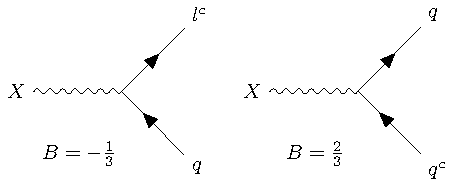
\includegraphics[width=0.7\textwidth]{Images/baryonnumber.pdf}
    \caption*{}
    \labfig{bnumber}
\end{figure}\\
In the case on the left, they couple to quarks and leptons so they are referred as \textbf{leptoquarks} while in the case on the right they transform quarks to antiquarks and they are called \textbf{diquarks}.\\
Consequently, through the mediation of a $X$ boson a $B=-1/3$ channel can be converted into a $B=2/3$ one, i.e. a baryon number changing process $(\Delta B=1)$ occurs at tree-level.\\
\begin{figure}[h]
    \centering
    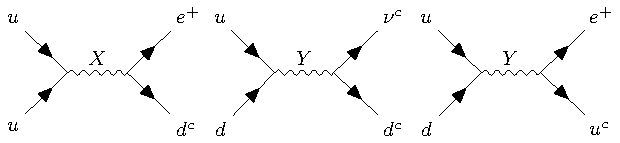
\includegraphics{Images/xyy.pdf}
    \caption*{}
    \labfig{xyy}
\end{figure}\\
$B-L$ is conserved, so a process like $p\to\pi^0e^+$ is allowed but not $n\to\pi^+e^-$. $B+L$ is instead violated, what are the operators accounting for such violation? These are dimension 6 $(B+L)$-violating operators:
\[
\frac{g^2_{\text{GUT}}}{M^2_{\text{GUT}}}u^{c\dagger}qe^{c\dagger}q \quad \frac{g^2_{\text{GUT}}}{M^2_{\text{GUT}}}u^{c\dagger}qd^{c\dagger}l 
\]
At Super-Kamiokande they measured $\tau(p\to\pi^0e^+)\ge1.4\cdot10^{34}$\,years resulting in $M_{\text{GUT}}\gtrsim10^{16}$\,GeV\marginnote[-2cm]{I am 0\% sure of what is written here because my notes on this part are terrible and there was someone using a drill in this exact moment so even the recording of the lecture is useless.}
\section{Custodial Symmetry}
Consider now the potential for the Higgs:
\[
V(H)=-\mu^2H^\dagger H+\lambda(H^\dagger H)^2 \quad H=\begin{pmatrix}\phi_1+i\phi_2\\\phi_3+i\phi_4\end{pmatrix}
\]
This is invariant under SO(4), $\phi_i\to\phi_i'=R_{ij}\phi_j$ with $RR^T=\mathbb{1}$. When $H$ acquires a vev, SO(4) is spontaneously broken to SO(3):
\[
\Braket{H}=\begin{pmatrix}0\\\frac{v}{\sqrt{2}}\end{pmatrix}\xleftrightarrow[]{}\Braket{\Phi}=\begin{pmatrix}0\\0\\\frac{v}{\sqrt{2}}\\0\end{pmatrix} \;\text{where}\;\Phi=\begin{pmatrix}\phi_1\\\phi_2\\\phi_3\\\phi_4\end{pmatrix}
\]
There exists an unbroken SO(3) that acts on entries 1,2 and 4 of $\Phi$. Remember that for SO$(n)$ there are $n(n-1)/2$ generators:
\[
\begin{cases}
n=4 \;\text{has 6 generators}\\
n=3 \;\text{has 3 generators}
\end{cases}
\Rightarrow 3\,\text{NGB}
\]
Looking at the algebras, we know that $\mathfrak{so}(3)\sim\mathfrak{su}(2)$ while the relation for SO(4) is given by $\mathfrak{so}(4)\sim\mathfrak{su}(2)\times\mathfrak{su}(2)$. It is also possible to write an exact relation of the previous one:
\[
\text{SO}(4)=\frac{\text{SU}(2)_{\text{L}}\times\text{SU}(2)_{\text{R}}}{\mathbb{Z}_2}
\]
Take now a vector of $\mathbb{R}^4$ denoted by $v^a$ which transforms under SO(4) as:
\[
v^a\to v'^a=R^{ab}v^b \quad a,b=1,2,3,4
\]
From this vector we can define $V:=v^aT^a$ where $T^a=\{i\Vec{\sigma},\mathbb{1}\}$ and $V$ is a $2\times2$ matrix. The transformation rule under SU$(2)_{\text{L}}\times$SU$(2)_{\text{R}}$ is the following:
\[
V\to V'=LVR^\dagger \quad L\in\text{SU}(2)_{\text{L}}, R\in\text{SU}(2)_{\text{R}}
\]
What is the connection with SO(4)? Compute the determinant of $V$:
\[
\det V=\det\left(\begin{array}{cc}
    v_4+iv_3 & iv_1+v_2 \\
    iv_1-v_2 & v_4-iv_3
\end{array}\right)=\sum_{i=1}^4(v_i)^2=\norm{\Vec{v}}^2
\]
When transforming $V$ under SU$(2)_{\text{L}}\times$SU$(2)_{\text{R}}$, the determinant remains the same therefore we have that $\norm{\Vec{v}}=\norm{\Vec{v}'}$. We can also define $v^a$ as:
\[
v^a:=\frac{1}{2}\Tr{T^{a\dagger}V}=\frac{1}{2}v^b\Tr{T^{a\dagger}T^b}=\frac{1}{2}v^b\delta^{ab}
\]
which transforms as:
\[
v'^a=\Tr{T^{a\dagger}V'}=\underbrace{\Tr{T^{a\dagger}LT^bR^\dagger}}_{:=R^{ab}}v^b
\]
The point is that for each element of SO(4) we have two elements of SU$(2)_{\text{L}}\times$SU$(2)_{\text{R}}$. SO(4) broken to SO(3) is the same as SU$(2)_{\text{L}}\times$SU$(2)_{\text{R}}$ broken to SU$(2)_{\text{V}}$ but this is something familiar: it is the chiral symmetry breaking in QCD with 2 flavours.\\
In the SM the masses of the $W$ and the $Z$ bosons are known and given by:\marginnote{From \cite{schwartz}, Section 31.2.}
\[
m_W^2=\frac{v^2}{4}g^2 \quad m_Z^2=\frac{v^2}{4}(g^2+g'^2)
\]
It turns out that $m_Z=m_W$ if $g'=0$ but it is not the case. However, their ratio is determined by the relative strengths of the weak and electromagnetic gauge couplings:
\[
\frac{m_W^2}{m_Z^2}=\frac{g^2}{g^2+g'^2}=\cos^2\theta_w
\]
This is a consequence of the way the SU$(2)\times$U(1) symmetry is spontaneously broken through the Higgs mechanism with a single SU(2) doublet. If the Higgs sector was more complicated, there might be deviations from this even at tree-level. It is therefore useful to define the $\rho$-parameter:
\[
\rho:=\frac{m_W}{m_Z\cos\theta_w}
\]
Denoting the tree-level value of $\rho$ as $\rho_0$ we see that $\rho_0=1$ in the Standard Model. What exactly guarantees that $\rho_0=1$? This is guaranteed by a symmetry and to see that recall that our original Higgs doublet $H$ transformed as a doublet under SU(2). Writing $H$ as:
\[
H=\frac{1}{\sqrt{2}}\begin{pmatrix}h_3+ih_4\\h_1+ih_2\end{pmatrix}
\]
we see that the potential becomes:
\[
V(H)=\lambda\left(H^\dagger H-\frac{v^2}{2}\right)=\frac{\lambda}{2}\left(h_1^2+h_2^2+h_3^2+h_4^2-v^2\right)^2
\]
This is actually invariant under a larger SO(4) symmetry under which the quadruplet $(h_1,h_2,h_3,h_4)$ transforms in the fundamental representation. Note that SO(4) has 6 generators while SU(2) has only 2. When $H$ gets a vev, such as $h_1=v$ and $h_2=h_3=h_4=0$, the SO(4) symmetry is broken to SO(3). There are actually three unbroken global symmetry directions in the Higgs sector of the SM. In other words, there is a residual global SU(2) symmetry after electroweak symmetry breaking which is known as \textbf{custodial isospin}, or \textbf{custodial SU(2)}.\\
In order to see corrections to the $\rho$-parameter, we can exploit the similarity with the Sigma model and rewrite the Higgs sector in terms of a new field $\pazocal{H}$:
\[
\pazocal{H}:=\frac{v+h(x)}{\sqrt{2}}\Sigma(x) \quad \Sigma(x)=\exp{i\frac{\chi^a\sigma^a}{v}}
\]
This is nothing but the product of the doublet $H$ and $H^c$ both seen as columns, i.e. $\pazocal{H}=[(H)(H^c)]$. In fact, it is possible to see that:
\[
\pazocal{H}^\dagger\pazocal{H}=\left(\begin{array}{cc}
    H^\dagger H & H^\dagger H^c \\
    H^{c\dagger}H & H^{c\dagger}H^c
\end{array}\right)=H^\dagger H\cdot\mathbb{1}\marginnote{This is because $H^{c\dagger}H^c=H^\dagger H$ and $H^{c\dagger}H=H^\dagger H^c=0$. Contino did not give much explanations about this, just \textit{convince yourself it is true} and \textit{prove it}.} 
\]
The potential can be now written in terms of $\pazocal{H}$ as follows:
\[
V(H)=-\frac{\mu^2}{2}\Tr{\pazocal{H^\dagger\pazocal{H}}}+\frac{\lambda}{4}\left(\Tr{\pazocal{H}^\dagger\pazocal{H}}\right)^2=-\frac{\mu^2}{2}(v+h)^2+\frac{\lambda}{4}(v+h)^4
\]
For the kinetic term instead we write:
\begin{align*}
\partial_\mu H^\dagger\partial^\mu H&=\frac{1}{2}\Tr{(\partial_\mu\pazocal{H}^\dagger)(\partial^\mu\pazocal{H}^\dagger)}\\
&=\frac{1}{2}(\partial_\mu h)^2+\frac{(v+h)^2}{4}\Tr{(\partial_\mu\Sigma^\dagger)(\partial^\mu\Sigma)}
\end{align*}
It turns out that it is possible to covariantize it and what we obtain is:
\[
D_\mu H^\dagger D^\mu H=\frac{1}{2}(\partial_\mu h)^2+\frac{(v+h)^2}{4}\Tr{(D_\mu\Sigma^\dagger)(D^\mu\Sigma)}
\]
where the covariant derivative is defined as:
\[
D_\mu\Sigma=\partial_\mu\Sigma-igW_\mu^a\frac{\sigma^a}{2}\Sigma+ig'\Sigma YB_\mu
\]
What is left to write is the Yukawa term, e.g. for quarks:\marginnote{For leptons is the same thing.}
\[
\pazocal{L}_{\text{Yuk}}\supset-q_L^iY_u^{ij}H^cu_R^j-\overline{q}_L^iY_d^{ij}Hd_r^j+\text{h.c.}=-\overline{q}_L^i\pazocal{H}\left(\begin{array}{cc}
    Y_u^{ij} & u_R^j \\
    Y_d^{ij} & d_R^j
\end{array}\right)+\text{h.c.}
\]
The fact that $m_u-m_d\neq0$ is another explicit breaking of SU$(2)_{\text{R}}$, hence of the custodial of SO(3). In particular, the most important effects come from top and bottom so we can consider the corrections at one-loop to the $W$ and $Z$ bosons coming from the virtual exchange of the top and bottom.
\begin{figure}[h]
    \centering
    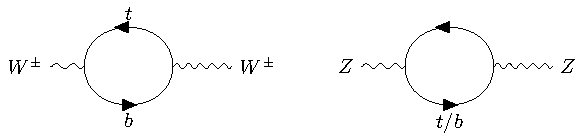
\includegraphics{Images/wztb.pdf}
    \caption*{}
    \labfig{wztb}
\end{figure}\\
If the masses of the top and the bottom were the same, these contributions would be the same but since the masses are different we have different corrections, $\delta m_Z\neq\delta m_W$. This implies $\Delta\rho\neq0$, in particular $\rho=1+\Delta\rho$. We can actually forget about the bottom, it is the top contribution which is relevant. $\Delta\rho\approx1/200$ which is in very good agreement with data, in fact experimentally we have $|\rho-1-\Delta\rho^{\text{SM}}|\lesssim10^{-3}$. This means that if we want to extend the SM we better not screw up with custodial symmetry because if we construct a new physics theory which violates at order one the custodial symmetry then that is ruled out. The custodial symmetry violation should be small, this is the message from data.\\
Since the custodial symmetry is an accidental symmetry, there should be some higher dimensional operators which accounts for its breaking. Which operator is breaking the symmetry? If we focus on the Higgs sector there is only one operator of dimension 6, given by $(H^\dagger\overset{\leftrightarrow}{D_\mu}H)^2$. In the unitary gauge, this would give a contribution to the mass of the $Z$ boson because the covariant derivative is sandwiched between two $H$ and we would get only the neutral component not the charged one. This means that custodial symmetry is violated.\\
There is another way to see that this operator breaks custodial symmetry. The theory can be reformulated in the following way:
\begin{align*}
\pazocal{L}=&\pazocal{L}_{\text{kin}}(\Psi)+\pazocal{L}_{\text{kin}}(\text{gauge})+\frac{1}{2}(\partial_\mu h)^2+\frac{(v+h)^2}{4}\Tr{(D_\mu\Sigma^\dagger)(D^\mu\Sigma)}\\
&-\overline{q}_L^i\Sigma\left(\begin{array}{cc}
    Y_u^{ij} & u_R^j \\
    Y_d^{ij} & d_R^j
\end{array}\right)\frac{(v+h)}{\sqrt{2}}+\text{h.c.}-V(h)
\end{align*}
Notice that $h(x)$ is a singlet of SO(4) so there is no covariant derivative here but we can think of $h$ as sort of the norm of $H^\dagger H$, which is an invariant of SU$(2)\times$U(1). We already saw a theory of this kind when we discussed the SU$(2)\times$SU(2) breaking in the previous course\marginnote{See \cite{EW}, Section 3.10 for more details about SU$(2)\times$SU(2) breaking.}. If we put only the three NGBs coming from the breaking then the scattering amplitudes at high energies grow and the theory becomes non perturbative. We then had to introduce an additional degree of freedom, the Higgs boson $h$, in such a way that the scattering amplitude coming from $\chi\chi\to\chi\chi$ would be exactly canceled by the Higgs contribution. This is because we introduced $h$ in this way and the way to see that this cancellation must occur is that we can rewrite this in terms of a renormalizable Lagrangian where there are no dimensionful couplings so there should be no dependency on the energy except for the usual running of the couplings. We did this thinking for example in terms of QCD. In QCD we can try the same, there are these three pions can we make things well behaved at high energies? We introduce an extra degree of freedom and we make a linear sigma model instead of a non-linear one. There is such a particle with the quantum numbers of the radial mode, which is the sigma particle, but this sigma particle does not couple in this way. First of all, it has a very large mass and second of all the mass is even complicated to define. If we do an experiment and see the resonance then it is really broad, that's why it is useful to define a mass, which means that eventually we will not have small couplings.\\
At the level of the global symmetry breaking pattern there is the same pattern but then the electroweak sector is including one degree of freedom which completes the theory into something renormalizable, while in the case of QCD this is not true. What happens? It happens that the theory becomes strongly coupled if we increase the energy. Consider a scattering at larger and larger energy, the theory is never unitarized perturbatively it becomes non perturbative. If we do the same scattering with $\chi$ then the amplitude grows but at a certain point it is saturated because there is the Higgs boson which turns on and the theory stays weakly coupled it does not become strongly coupled. Experimentally, how precisely do we know the Higgs coupling? It seems that having couplings exactly equal to those of this Lagrangian is crucial because otherwise if we start changing these couplings the cancellation does not occur anymore. So the question is: \textit{does the Standard Model reproduce nature or not?} The couplings could be equal to the SM values plus small corrections. How can we write a theory where the Higgs boson has a different coupling? We can simply relax some of our assumptions, here the assumption is that the SU$(2)_{\text{EW}}\times$U$(1)_{\text{Y}}$ symmetry is realized linearly at high energies, at $E\gg v$ we can forget about the breaking and the symmetry is realized linearly so all the fields have to come in multiplets of this symmetry. We could in principle relax this so what we need to account for is the fact that the $W$ and the $Z$ bosons are massive, that's the experimental evidence. Of course we need to have this symmetry which is be spontaneously broken, there should be the Higgs mechanism, everything is the same but we do not need to ask for a linear realization at high energies. We could completely eliminate the Higgs boson from the theory, and that's basically what we have in technicolor theories, or we can introduce it but without requiring that the symmetry is realized linearly. This means that we need to construct a Lagrangian which has the global symmetry SU$(2)\times$SU(2) broken to SU(2) and then we gauge the subgroup, we do not impose that it has to reconstruct linear multiplets. Considering all terms which are invariant under the symmetry, the most general Lagrangian we can write is:
\begin{align*}
\pazocal{L}=&\pazocal{L}_{\text{kin}}(\Psi)+\pazocal{L}_{\text{kin}}(\text{gauge})+\frac{1}{2}(\partial_\mu h)^2\\
&-\frac{v}{\sqrt{2}}\overline{q}_L^i\Sigma\left(\begin{array}{cc}
    Y_u^{ij} & u_R^j \\
    Y_d^{ij} & d_R^j
\end{array}\right)\left(1+c_q\frac{h}{v}+\cdots\right)\\
&+\frac{v^2}{4}\Tr{(D_\mu\Sigma^\dagger)(D^\mu\Sigma)}\underbrace{\left(1+2c_v\frac{h}{v}+c_{2v}\frac{h^2}{v^2}+\cdots\right)}_{\text{singlet of SU$(2)\times$SU(2)}}-V(h)
\end{align*}
where the potential is given by:
\[
V(h)=-\frac{m_h^2}{2}h^2(x)+c_3\frac{m_h^2}{6v}h^3(x)+c_4\frac{m_h^2}{v^2}h^4(x)+\cdots\marginnote{Maybe in literature $c_3$ and $c_4$ are called $\lambda_3$ and $\lambda_4$.}
\]
In the SM limit, $c_v=1$ and $c_{2v}=1$. In other words, these two parametrize the following interactions:
\begin{figure}[h]
    \centering
    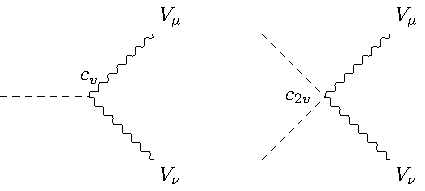
\includegraphics[width=0.7\textwidth]{Images/cvc2v.pdf}
    \caption*{}
    \labfig{cvc2v}
\end{figure}\\
This Lagrangian makes sense because it is invariant under SU$(2)\times$U(1), of course only for these values we can reconstruct the Higgs boson but for values of these parameters different from 1 we still have gauge invariance but the symmetry is not realized linearly not because of a lack of degrees of freedom. For the other parameters, the SM is realized for $c_q=1$, $c_3=1$ and $c_4=1$. The theory is not renormalizable so it will blow up at a certain point but who cares, it is an EFT but we knew it from the beginning. Where is the cut-off? Here it has to be, without a doubt, a few TeV because that is the energy at which couplings blow up. This is the \textbf{non-linear electroweak Lagrangian} and it is constructed by making fewer assumptions than the SM, we ask for SU$(2)\times$U(1) symmetry but we do not ask for linearity.\\
Somebody may complain: the kinetic term we wrote for $\Sigma$ is the term which follows if we impose an invariance under SU$(2)\times$SU(2) and then we gauge SU$(2)\times$U(1). However, here the custodial symmetry is not imposed by hand, we do not want to say that it is necessarily recovered if we switch off the gauging. That was true for the linear Lagrangian, because the first operator which breaks custodial symmetry arises at dimension 6 level. In that case, custodial symmetry was accidental at low energy, is it true also here? The answer is no, because if we do not impose that by switching off the gauging we recover custodial symmetry then there is another kinetic term that we can write. Remember that the rule of this game is that we have to have local invariance under SU$(2)\times$U(1) but we are not imposing custodial symmetry. If we do not impose custodial symmetry then there is another term that we can write which is invariant only under SU$(2)\times$U(1). How can we write it? First of all let's recall that $\Sigma$ transforms as $\Sigma\to L\Sigma R^\dagger$ with $L\in\text{SU}(2)_{\text{L}}$, $R\in\text{SU}(2)_{\text{R}}$ and hypercharge is the third generator of SU$(2)_{\text{R}}$. It is then possible to construct the following objects:
\[
\Sigma^\dagger D_\mu\Sigma\to R(\Sigma^\dagger D_\mu\Sigma)R^\dagger \quad \Sigma D_\mu\Sigma^\dagger\to L(\Sigma D_\mu\Sigma^\dagger)L^\dagger
\]
The kinetic term can also be rewritten as:
\[
\Tr{D_\mu\Sigma^\dagger D^\mu\Sigma}=\Tr{\Sigma^\dagger D_\mu\Sigma\sigma_3\Sigma^\dagger D_\mu\Sigma\sigma_3}
\]
It is clear that we have one of these two objects and we are making the square and then we take the trace. Of course we can take either the right-handed or the left-handed term, it is the same. The other kinetic term comes from by noticing that there has to be invariance under SU$(2)_{\text{L}}$ but we do not impose invariance under SU$(2)_{\text{R}}$ and only invariance under U$(1)_{\text{Y}}$ which is inside SU$(2)_{\text{R}}$. We can also write a double trace operator:
\[
\left[\Tr{\Sigma^\dagger D_\mu\Sigma\sigma_3}\right]^2\frac{\alpha_Tv^2}{8}
\]
Without putting the $\sigma_3$ matrix this operator would be 0 because we can easily show that the trace of such quantity is 0. This term is invariant under SU$(2)_{\text{L}}\times$U$(1)_{\text{Y}}$ but not under SU$(2)_{\text{L}}\times$SU$(2)_{\text{R}}$ and it breaks custodial symmetry. If we now go to the unitary gauge where $\Sigma$ is equal to the identity, from the trace of the covariant derivative times $\sigma_3$ we get the mass terms of the $W$ and $Z$ bosons:
\[
m_W^2=\frac{v^2}{4}g^2 \quad m_Z^2=\frac{v^2}{4}(g^2+g'^2)v^2(1+\alpha_T)\Rightarrow\rho=\frac{1}{1+\alpha_T}\neq1
\]
Why such a term was not appearing in the linear realization? Well it is appearing but at dimension 6. The point is that incorporating the fourth degree of freedom into a Higgs doublet forces this effect arising at dimension 6. Custodial symmetry in this formulation does not appear as accidental, this breaking is at the same order of the kinetic term and the parameter $\alpha_T$ has to be very small. The Lagrangian is an effective one which means that at the scale at which we integrate out the new physics then we get this Lagrangian and at that scale this coefficient has to be small. It is an effective description of our physics valid up to a certain cut-off scale at which we integrate out the heavy fields. Because this UV dynamics respects the custodial symmetry, this parameter will be small. Then we do experiments at low energy so this parameter $\alpha_T$ would run and we see radiative corrections from UV effects. The point is that if we allow the UV dynamics to be completely general then this $\alpha_T$ would be of order 1 and the $\rho$-parameter would be too large, therefore we have to assume whatever physics we are integrating out has to be custodial invariant to a very good degree, corrections must be very small.\\
Let's clarify a bit which is the expansion we are assuming. There is a double expansion. First, similarly to the chiral Lagrangian in QCD, there are high order terms which involve a number of derivatives divided by the currents. These terms would give us effects of order energy at which we do experiments divided by $\Lambda$. Notice that here we are not expanding in power of the fields divided by $\Lambda$ because fields might have dimensionality zero. We are expanding in derivatives divided by $\Lambda$ and then of course we are also expanding in the number of Higgs boson fields. This is not really an expansion but it is a way to organize the terms so at a certain Higgs order in the number of $H$ fields we have a finite number of terms but it is clear that the more Higgs fields we have the larger will be the number of Higgs particles involved in our process. E.g. if we have a process with only one Higgs field, then we can stop at the level of one Higgs field in the Lagrangian. This is not true if we have the Higgs doublet, because it acquires a vev so if we have ten of these fields we can still get a contribution zero to a process with zero physical Higgs bosons, simply by putting vev in all these fields. While here we separated the vev from the physical excitation so the more fields $h$ we have the more Higgs particles there will be in our process. Plus we have an expansion in derivatives, this is the double expansion we have.\\
Notice that if we compare with the linear Lagrangian which is a function of $H$ this also has to be thought as an EFT so we have the terms with dimension 4 plus terms with higher dimension. Here indeed we are expanding in numbers of fields because every time we put a field it has dimension 1 so we expand in the number of derivatives and also in the number of fields because they give us the dimensionality. However, the matching is not straightforward because an operator which obtains a certain number of $H$ fields does not correspond to a single operator.
\begin{figure}[h]
    \centering
    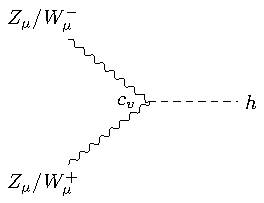
\includegraphics[width=0.45\textwidth]{Images/zwcv.pdf}
    \caption*{}
    \labfig{zwcv}
\end{figure}\\
For example, this gives a cubic interaction between the Higgs and the vector boson, the interaction vertex is modified by the parameter $c_v$. How can we modify the same interaction in the linear formulation? There will not be any term at dimension 4 because those are the terms of the SM so they have to be terms coming from higher dimension operators. Corrections to this vertex come from dimension 6 operators. In the assumption of only 1 family, at $D=5$ there is only one operator, the Weinberg one, but at $D=6$ there are 59 operators, which are a lot. Some of them were considered even before studying the Higgs physics, e.g. $(H^\dagger D_\mu H)^2$ gives $\Delta\rho$ which has not necessarily anything to do with the Higgs physics. On the other hand, some of them modify \textit{only} the Higgs physics and before the discovery of the Higgs at LHC they were not testable.
\[
O_{WW}=H^\dagger HW_{\mu\nu}^iW^{\mu\nu,i} \quad O_{BB}=H^\dagger HB_{\mu\nu}B^{\mu\nu} \quad O_{GG}=H^\dagger HG_{\mu\nu}^aG^{\mu\nu,a}
\]
If we set $H$ to the vev, they give us some terms which are already present in the Lagrangian. For example, $O_{WW}$ gives the kinetic term of the $W$ in this way. These operator gives cubic interaction but not of the form seen before because they now give vertices with two derivatives.
Then there is another one of the form:
\[
O_H=[\partial_\mu(H^\dagger H)]^2\supset v^2(\partial_\mu h)^2
\]
which vanishes if we set $H$ to the vev and it is only modifying the kinetic term of the Higgs boson. Since it gives a correction to the kinetic term if we renormalize it then this correction will appear in all vertices.
\[
|D_\mu H|^2+c_HO_H\supset\frac{1}{2}\left(1+\frac{c_Hv^2}{2}\right)(\partial_\mu h)^2\marginnote{$c_H$ has dimension $-2$.}
\]
This means that it is possible to redefine $h(x)$ and get:
\[
h(x)\to\frac{h(x)}{\sqrt{1+\frac{c_Hv^2}{2}}}\simeq\left(1-\frac{c_Hv^2}{4}\right)h(x)
\]
The point is that since we want to normalize canonically the kinetic term, then in every vertex where there is a factor $h$ then we will get this factor here and this is universal, it is a modification to any coupling in the same way. In particular, $c_v$ will get a contribution from $O_H$:
\[
c_v=1-\frac{c_Hv^2}{4}
\]
At dimension 6 there are other operators which modify the couplings of the fermions, because we can write operators of this form:
\[
O_\Psi=H^\dagger H\overline{\Psi}_LH\Psi_R
\]
where $\Psi$ is either a quark or a lepton. This will give us the correction to the coupling of fermions with the Higgs field.
\begin{figure}[h]
    \centering
    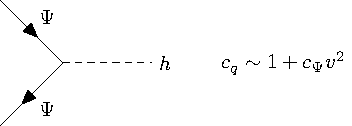
\includegraphics[width=0.6\textwidth]{Images/cq.pdf}
    \caption*{}
    \labfig{cq}
\end{figure}\\
Then there is an operator called $O_6$ of the form:
\[
O_6=(H^\dagger H)^3
\]
which affects the potential, i.e. the Higgs self interaction, in particular it will modify the cubic and quartic interaction and generates higher order interactions involving 5 or 6 Higgs bosons which are really impossible to detect experimentally. The 4 Higgs bosons interaction is already beyond the physics that we in this room can see.\marginnote{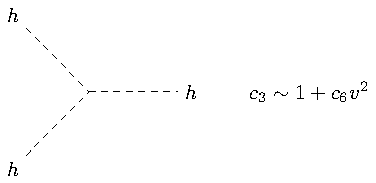
\includegraphics[]{Images/c3.pdf}}\\
There are other three operators which are CP-odd, e.g. $H^\dagger HW_{\mu\nu}\Tilde{W}^{\mu\nu}$. All these operators affect only the Higgs physics and can modify the Higgs coupling, so if we have the linear Lagrangian the modification to the Higgs coupling arise at the dimension 6 level. However, we get corrections also from $D=8$ operators. For example, we can consider:
\[
O_{2H}=H^\dagger H[\partial_\mu(H^\dagger H)]^2
\]
Clearly, this operator will give us a shift in the Higgs coupling:
\[
c_v=1-\frac{c_Hv^2}{4}+c_{2H}v^4+(\;\;)v^6+(\;\;)v^8+\cdots\marginnote{$c_{2H}$ has dimension $-4.$} 
\]
At this point we can understand what is the relation between the linear and non-linear Lagrangian: in the linear Lagrangian, these coefficients scale like:
\[
c_H\sim\frac{g_*^2}{m_*^2} \quad c_{2H}\sim\frac{g_*^4}{m_*^4}
\]
where $g_*$ and $m_*$ are the coupling and the mass characterizing the new physics. The point now is whether such a quantity explode or not and this depends on the scale of new physics. Obviously there are two different possibilities depending also on the value of $g_*$ which characterizes the strength with which the Higgs bosons interacts with the new physics, so the stronger this interaction is the more important the corrections will be. In the limit of technicolor, which is a theory in which everything is strongly interacting, this ratio is really of order 1. There is no hierarchy between the numerator and the denominator, resonances appear at this scale. If the new physics is strongly interacting and all these terms are important, then we cannot really use the linear realization because the cut-off scale is too small compared to $g_*$. In fact, $g_*\sim4\pi$ is exactly what we have if we do not put the Higgs boson. This is the case in which this new physics is strongly interacting and the scale is such that the ratio is really of order 1. Therefore we have to use the non-linear Lagrangian which, in a sense, re-sums all these terms. Such terms are terms in which we expand in powers of $g/m_*$ so this single coupling encodes the effect of all these higher dimension operators. But since we do not have a separation of scales we cannot really expand in the linear regime. Instead, if the cut-off of the new physics appears at a scale which is large enough and weakly coupled then at this point it will be possible to truncate this series because the higher in the dimension we go the more suppressed the effects will be.\\
It is important to say something about how strong the new physics is, not just at which scale it appears but also if it is strongly or weakly coupled. Strongly coupled physics at small energy implies that the linear realization does not occur. Linearly realized symmetry instead requires a gap and the new physics remains weakly coupled up to the cut-off scale, there is a regime in which the theory is weakly coupled. Of course some of these dimension 6 operators will involve more derivatives and they will map into operators, in the non-linear Lagrangian, involving more derivatives.\\
This is not easy to digest but it is important to do it because there are these two mathematical descriptions and now we have to describe data, so we have to know how to use these descriptions. Depending on the data, one of the descriptions might be good and the other might not be useful. In particular, if the new physics was technicolor then we should have used this (?) Lagrangian because there was no possible expansion in the linear formalism. On the other hand, if there were no evidence of technicolor then the linear Lagrangian would be a good description.\\
Remember that this is an EFT, so we integrate out the heavy physics and match the full theory with the heavy theory. This gives us the value of $\alpha_T$ and other parameters at the scale we are doing matching, at least at high scale $\alpha_T$ has to be small. What does it mean that it is small at the cut-off scale? It means that the degrees of freedom we are integrating out respects custodial symmetry, the new physics has to be custodial invariant. Here the situation is better at the linear level because custodial symmetry already appears as accidentally. As long as there is a gap between the energy at which we do experiments and the cut-off scale then this effect is automatically small but we might be in the other situation and not getting the benefits of accidental custodial symmetry, we have to somehow impose it at the level of the new physics. Notice that the presence of this term is exactly what differentiates the two possible different patterns of global symmetry breaking.
\[
\begin{aligned}
&\alpha_T=0: &&\text{SU$(2)_{\text{L}}\times$SU$(2)_{\text{R}}\to$SU$(2)_{\text{V}}$}\\
&\alpha_T\neq0: &&\text{SU$(2)_{\text{L}}\times$U$(1)_{\text{Y}}\to$U$(1)_{\text{EW}}$}\\
\end{aligned}
\]
These two possibilities correspond to two different patterns of global symmetry breaking. Both patterns will give us 3 NGBs which will have to transform, as usual, as the representation of the unbroken group. In the first case, the 3 NGBs are 3 irreps, so an adjoint of SU$(2)_{\text{V}}$. In the second case instead, they are reducible representations denoted by $\chi^\pm$ and $\chi^0$ and that is why we can write two kinetic terms, one for each reducible representation. If we enlarge the pattern of symmetry breaking, for example at the classical level, and if we include the Goldstone bosons that come from the spontaneous breaking of U$(1)_{\text{A}}$\marginnote{Forget for a moment about the anomaly.} then we will have two kinetic terms with two unrelated coefficients. This is important in the limit of large number of colours because in that case the anomaly switches off. Every time the Goldstone bosons form reducible representations, with respect to the broken group, then each reducible representations has its own kinetic term. The fact that experimentally the custodial symmetry is an approximate symmetry of our world implies that up to small effects these 3 NGBs are transforming very closely to an irreducible representation of SU$(2)_{\text{V}}$, that is the custodial symmetry. 
\section{Scattering Amplitudes at High Energies}
Before discussing the Higgs physics and how the Higgs boson decay we want to analyze a bit what happens to the scatterings for generic Higgs couplings. We have said that this theory is effective, is not a complete one and this means that there must be some process whose cross section blows up when we go at high energy so the theory cannot be maintained at perturbative regime. Which scattering amplitudes should we consider? Let's first analyze the role of the coupling $c_v$ which corresponds to two vector bosons going to one Higgs.\\
\begin{figure}[h]
    \centering
    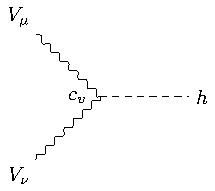
\includegraphics[width=0.4\textwidth]{Images/cvvv.pdf}
    \caption*{}
    \labfig{cvvv}
\end{figure}\\
We should remember from the previous course\marginnote{Previous course=\cite{EW}.} that the exchange of the Higgs in the $WW$ scattering amplitude was crucial to restore perturbative unitarity, so one amplitude that we should monitor is $W^+W^-\to W^+W^-$.\\
\begin{figure}[h]
    \centering
    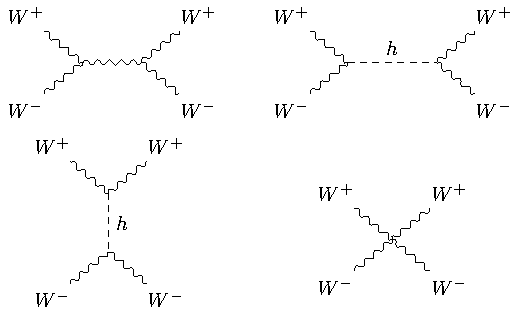
\includegraphics[width=0.8\textwidth]{Images/wwww.pdf}
    \caption*{}
    \labfig{wwww}
\end{figure}\\
The total amplitude goes like:
\[
A=\frac{1}{v^2}\left[s-\frac{s^2}{s-m_h^2}c_v^2+(s\leftrightarrow t)+\cdots\right]\underset{\mathclap{\tikz \node {$\uparrow$} node [below=1ex] {\footnotesize  $s\to\infty$};}}{\simeq}\frac{s}{v^2}(1-c_v^2)+(s\leftrightarrow t)+\cdots
\]
There is a contribution which grows with the energy coming from the sum of the pure $W$ diagrams, and it is the term $s/v^2$, but then there is the contribution from the Higgs exchange with the $c_v^2$ factor coming from the fact that there are two couplings. The $\cdots$ denote finite terms which do not grow with the energy. If we want to cancel this growth with the energy, we have to set $c_v=1$, that is the way to cure the loss of perturbativity. This is the Standard Model point, it is a bottom-up way to derive the SM.\\
Then there is also the coupling $c_{2v}$, the coupling of two Higgs with two $W$. In order to constrain that, we have to consider the following scatterings processes.\\
\begin{figure}[h]
    \centering
    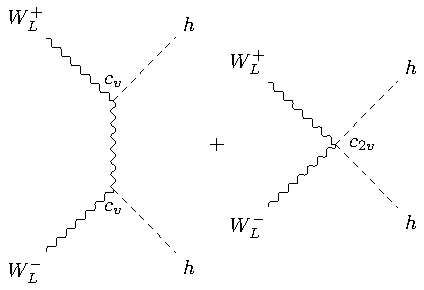
\includegraphics[width=0.6\textwidth]{Images/wlh.pdf}
    \caption*{}
    \labfig{wlh}
\end{figure}\\
At high energy, this amplitude goes like:
\[
A\simeq\frac{E^2}{v^2}(c_{2v}-c_v^2)+\cdots
\]
Again, we have to set $c_{2v}=1$ in the SM so that the amplitude does not explode. Why does the sum of these terms go like $E^2$? Because the polarization goes like one power of the energy, $\varepsilon_\mu^L=\frac{p_\mu}{m_W}(1+\pazocal{O}(m_W^2/E^2))$. We have two of these objects, the coupling has no derivatives so the amplitude goes like $E^2$.\\
In this story it is very useful to use the equivalence theorem, which tells us that we can simplify the calculation by replacing the longitudinal $W$ with the would-be Goldstone bosons which interact with the Higgs through the chiral Lagrangian when we switch off the gauging. For example for this process we have:\\
\begin{figure}[h]
    \centering
    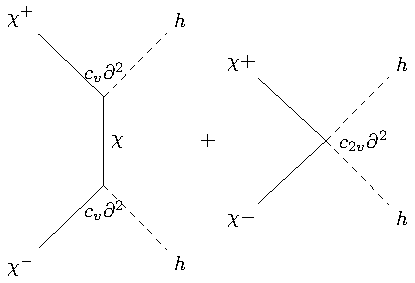
\includegraphics[width=0.7\textwidth]{Images/chih.pdf}
    \caption*{}
    \labfig{chih}
\end{figure}\\
Now, there is no energy factor coming from the polarization vector but there are derivatives in the vertices. The diagram on the left in particular gives four powers of the energy from the vertices, $1/v^2$ from the propagator so again it is proportional to $v^2$ and there are two powers of $c_v$. The simplification we get by using the equivalence theorem is more evident if we look at $WW$ scattering where there is sum over diagrams involving only the $W$ bosons and the equivalence theorem maps everything into just one diagram where the vertex goes like two derivatives. Here the equivalence theorem is very useful because each diagram naively goes like $E^4$ since there are 4 longitudinal $W$. For the diagram relative to the contact interaction this is easy to see, for the process with the propagator there is a factor $E^4$ coming from polarizations, $E^2$ coming from the vertices and then the propagator which in the unitary gauge goes like $E^0$ so in the end it will go like $E^6$. However, if we sum all these diagrams then we find that there is a cancellation and this sum goes like $E^4$. Now if we sum everything, the total goes like $E^2$ because there is another cancellation. In addition to that, we have to add the contribution of the Higgs which goes like $E^2$ so in the SM there would be another cancellation. It is clear that all this calculation would be way easier by using the equivalence theorem. When we want to use these tools to parametrize the Lagrangian, we keep the couplings $c_v$ and $c_{2v}$ generic and there would be no cancellation in the diagrams involving interactions between the Higgs and the $W$.\\
In order to constraint the coupling $c_q$, we look at the scattering of $W$ bosons into quarks, i.e. $W_L^+W_L^-\to q\overline{q}$.
\begin{figure}[h]
    \centering
    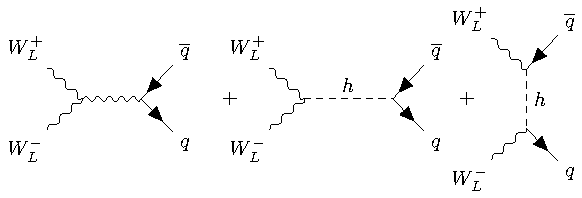
\includegraphics{Images/wwqq.pdf}
    \caption*{}
    \labfig{wwqq}
\end{figure}
There is a factor $E^2$ coming from the $W$ bosons, there is a $\sqrt{E}$ coming from each spinor and in the unitary gauge there is no derivative so it will be proportional to a factor $m_q/v^2$ and finally $1/E^2$ coming from the propagator so this diagram goes like:
\[
E^2(\sqrt{E})^2\frac{m_q}{v^2}\frac{1}{E^2}\sim E\frac{m_q}{v^2}
\]
The growth is not like $E^2$ but instead is proportional to one power of the energy times the mass of the quark which means that in order to better see this effect we should consider the top quark. Using the equivalence theorem, we obtain an interaction involving $\Sigma$, $q$ and also the Higgs. By expanding $\Sigma$, which is $\exp{i\chi^a\sigma^a/v}$ then we get:
\[
\overline{q}_L\Sigma q_R\left(1+c_q\frac{h}{v}+c_{2q}\frac{h^2}{v^2}+\cdots\right)\simeq\overline{q}_Lq_R(1+\chi+\chi^2+\cdots)
\]
This is a contribution which couples directly two $\chi$ with $q\overline{q}$ and goes like $m_q(\sqrt{E})^2/v^2$. Notice that these quarks have opposite helicity, of course there are different scatterings, e.g. we can consider $\chi\chi\to q_Lq_R$ or $\chi\chi\to q_Lq_L$ or $\chi\chi\to q_Rq_R$. The process which goes like $E^2$ is the one involving left- and right-handed.\\
There is a left-right invariance of the chiral Lagrangian under which we exchange left- and right-handed. At the level of $\Sigma$, the axial generators in the exponential get a minus sign and we can also say the same thing by transforming the fields instead of the generators so under this symmetry $\chi\to-\chi$. The vertices which come out of this interaction have to involve an even number of $\chi$ bosons. The possible diagrams are then given by:
\begin{figure}[h]
    \centering
    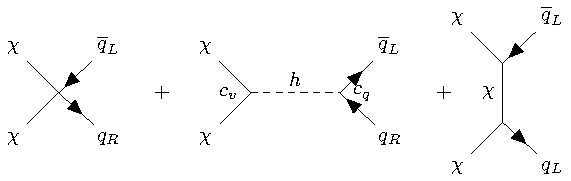
\includegraphics{Images/chichiqq.pdf}
    \caption*{}
    \labfig{chichiqq}
\end{figure}\\
Looking at the amplitude of the diagram on the right, this goes like $(\sqrt{E})^21/E\sim E^0$ and as we can see it does not grow with the energy. If we select the scattering of $\chi\chi$ going into two left-handed quarks then the amplitude does not grow with the energy, if we select instead left- and right-handed quarks then we will get something which grows like $E$. But there is also a contribution from the Higgs with an amplitude going like $E^2(\sqrt{E})^21/E^2$. Summarizing, using the equivalence theorem in the $\xi$-gauge we are left with the contributions of the first two diagrams, i.e. $\chi\chi\to\overline{q}_Lq_R$.
\[
A(\chi^+\chi^-\to\overline{q}_Lq_R)\propto\frac{m_qE}{v^2}(1-c_vc_q)+\cdots
\]
This has to be 0 in the SM, which implies that $c_q=1$ since we already constrained $c_v$ to be equal to 1.\\
There are other couplings that we can consider, for example the triple Higgs coupling. This coupling by itself does not involve a growth with the energy in the scattering amplitude, it does not give any problems because there is no cancellation in scattering amplitudes which is ruined by this parameter. There are other interactions instead more problematic, e.g. we can look at $c_{2q}$ which is the coupling of $q\overline{q}$ with two Higgs.
\begin{figure}[h]
    \centering
    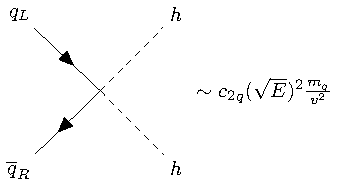
\includegraphics[width=0.6\textwidth]{Images/c2q.pdf}
    \caption*{}
    \labfig{c2q}
\end{figure}\\
It is not something that can be easily done experimentally but it exists on the theoretical side. If $c_{2q}$ was different from zero it would create a growth with the energy so we have to impose that $c_{2q}=0$ because otherwise there is a single contribution from this scattering which grows with the energy.\\
The fundamental question is: \textit{how much can we extrapolate of a theory given the knowledge of the precision that we have on the Higgs couplings?}\\
The precision on the Higgs coupling is:
\[
\frac{\delta g_h}{g_h}\approx10\%
\]
This number is an over-simplification, there are some couplings which are better and other couplings which are not even known. As we will see, it depends on how we do the fit. We have a certain set of experimental data that we have to fit with some theoretical predictions and this depends on how many assumptions one makes. For example, if we make a super generic fit then there will be so many couplings that we will not be able to fit so there is the need to make some simplifications. One possible simplification is the one in which one says \textit{okay let me consider the possible situation in which are the couplings are shifted by a single common parameter}, e.g. if the only operator we turn on is $O_H$ that is exactly the case, a universal shift to all the couplings. The precision that we get on this deviation is better than 10\%, is (4-5)\%. In this picture, we have that at the electroweak scale $\pazocal{O}(100$\,GeV) we can extrapolate the theory up to which point? Suppose we take any of these couplings and make them different from the SM prediction, what do we get? An amplitude which goes like:
\[
A(WW\to WW)\propto\frac{E^2}{v^2}(1-c_v^2)\simeq\delta c_v\frac{E^2}{v^2}\Rightarrow E\lesssim\Lambda=\frac{4\pi v}{\sqrt{\delta c_v}}
\]
This is because perturbative unitarity is loss when the amplitude is of order of $16\pi^2$. The theory will become non-perturbative and non-unitary at this scale and new physics has to come essentially before this scale. It is then possible to extrapolate up to energy of this order. If we assume $\delta c_v$ of order 10\% then we get $\Lambda\approx10$\,TeV. The answer is that the knowledge we have on these couplings justifies the extrapolation of the theory up to energy of order 10 TeV in a weak regime. If the couplings are closer to the SM predictions then perturbative unitarity holds true for longer and the sooner new physics appear, the weaker can be.\\
It is possible to repeat the story for a theory without the Higgs, in this case there will be $\Lambda=4\pi v$ and scattering amplitudes at this scale will blow up. New physics has to come before $\Lambda$ and in this case it would be the Higgs, in fact when they were looking for the Higgs before its discovery they did not know where the mass was and they were saying \textit{okay, if the Higgs is as far as 1 TeV it is so heavy that the theory is very strongly coupled}. It turned out that the Higgs was lighter so the theory is weakly coupled.\\
In the SM point, in principle we can extrapolate the theory to very very high energies without having problems with scattering amplitudes however the couplings will run logarithmically and again we might have a loss of perturbativity due to the fact that some of the couplings blow up. There are two possible couplings which can blow up: the quartic coupling of the Higgs and the one relative to the hypercharge.\marginnote{The point is that it blows up at $10^{42}$\,GeV so we do not care.}  Consider now the SM, which has a potential given by:
\[
V(H)=-\mu^2(H^\dagger H)+\lambda(H^\dagger H)^2
\]
The coupling $\lambda$ will have contributions from itself and from the top quark:\marginnote[-1cm]{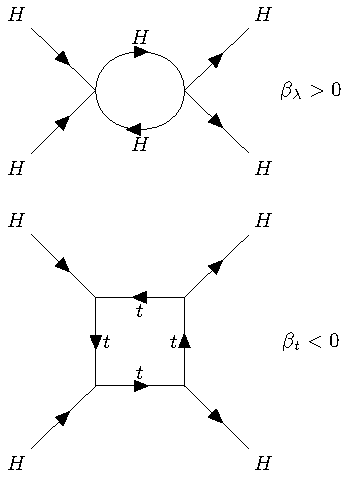
\includegraphics[]{Images/betatbetal.pdf}\\
Contributions for $\beta_\lambda$ and $\beta_t$.}
\[
\mu\frac{d}{d\mu}\lambda=\frac{\beta_\lambda}{16\pi^2}\lambda^2+\frac{\beta_t}{16\pi^2}y_t^4
\]
$\beta_\lambda$ is positive but $\beta_t$ is negative. Notice that $\lambda$ morally is the coupling squared, loss of perturbation theory occurs for $\lambda$ of order $16\pi^2$. There are two compelling effects in this story and it depends on the initial condition: if we start with a very small value of $\lambda$, i.e. light Higgs, then the first term would be subleading with respect to the top term which will win and the coupling will decrease as we go up in energy. On the other hand, if $\lambda$ at the initial point is large, i.e. heavy Higgs, then the first term will dominate, the coupling will increase by running up in energy and perturbative unitarity will be lost at a certain point. It turns out that the Higgs is light so the first term is subleading, the initial conditions are so small that the top ends up winning. The coupling decreases with the energy and there is a very very high energy at which $\lambda$ crosses the zero and becomes negative. One might now be worried that a negative $\lambda$ corresponds to a potential which is unbound from below.\marginnote{There is a connection between the evolution of $\lambda$ as a function of the energy and the stability of the vacuum, but it is a bit technical so I will skip it.}
%La roba a bit technical sta da 1:27:43 in poi lezione del 05/12
\section{Higgs Physics at LHC: an Overview}
\subsection{Production}
How can we produce a Higgs boson? It has to come from the interaction of particles with sufficiently high energy. At LEP they tried with $e^+e^-\to Zh$,
% \begin{figure}[h]
%     \centering
%     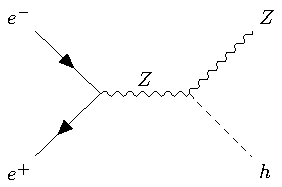
\includegraphics[width=0.45\textwidth]{Images/higgslep.pdf}
%     \caption*{}
%     \labfig{higgslep}
% \end{figure}\\
this process requires having an invariant mass of $\sqrt{s}>m_h+m_Z$ and there was not enough energy to make it happen. At LHC more energy was available but it is a much more complicated environment: basically protons are smashed together. Protons are composite particles made of three quarks as we know and $\sqrt{s}$ was 7 TeV at the time of the discovery, then it went up to 8 TeV and finally to 13 TeV. The first two values correspond to Run 1, the latter to Run 2. Run 3 just started with increased energy but analyzed data from Run 3 are not available yet, so the results will come from Run 1 and Run 2 and we will consider the integrated luminosity of Run 2 much larger than the one of Run 1.\\
How can the Higgs boson be produced at LHC? It has couplings with the quarks so the process is the following:
\begin{figure}[h]
    \centering
    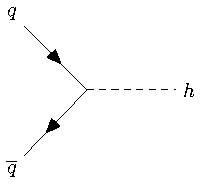
\includegraphics[width=0.35\textwidth]{Images/qqhiggs.pdf}
    \caption*{}
    \labfig{qqhiggs}
\end{figure}\\
However, this vertex is proportional to $m_q/v$ so it is large if we have the top quark but unfortunately the top quark is not one of the valence quarks. But in addition to the valence quarks there are also the sea quarks, i.e. quarks that are produced by fluctuations in the vacuum coming from the facts that these quarks radiate  virtual gluons which split and in principle it is possible to have everything. We can even think of having a top out of this but it is very difficult, it has a very small probability to happen. Creating a bottom is more feasible, the probability of having a bottom inside a proton is not entirely negligible. It turns out that at the energy of the LHC, the probability to get a gluon inside the partons is very large, so one of the main process that it is possible to have is \textbf{gluon-gluon fusion} (GGF). These two gluons can meet and interact: 
\begin{figure}[h]
    \centering
    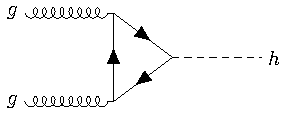
\includegraphics[width=0.45\textwidth]{Images/ggf.pdf}
    \caption*{}
    \labfig{ggf}
\end{figure}\\
In the loop, the top quark will give the largest contribution. Despite the fact that this is a one-loop effect, it gives the largest cross section at LHC.\\
Then there is the coupling with vector bosons, however extracting the $W$ from the proton is difficult and very very rare. We then start with quarks and radiate a $W$ from the quarks, so the process which goes under the name of \textbf{vector boson fusion} (VBF) is:
\begin{figure}[h]
    \centering
    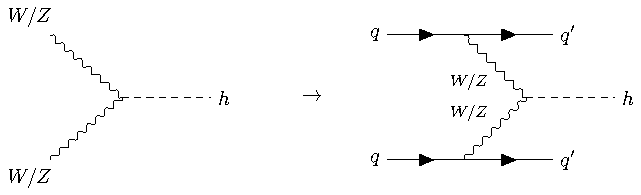
\includegraphics[width=0.8\textwidth]{Images/vbf.pdf}
    \caption*{}
    \labfig{vbf}
\end{figure}\\
Here the final state is not just the Higgs but the Higgs plus two quarks and it turns out that these quarks are very forward. Normally we have an interaction along the $z$-axis and the products in the final state have a certain distribution but particles that are very close to the beam line are more difficult to detect because there is other stuff which goes forward: two quarks can interact but the rest of the protons travel and hit the detector as well in the forward direction. It is much more clean to look at what happens in the transverse direction.\\
VBF has a cross section which is way smaller than GGF because we need to have a $W$ or $Z$ boson radiated from the quarks, there are couplings involved. It is true that in GGF there is a loop but the couplings are strong and they are larger than the ones in VBF.\\
There is also associated Higgs production which is when we have $q\overline{q}\to W/Zh$:
\begin{figure}[h]
    \centering
    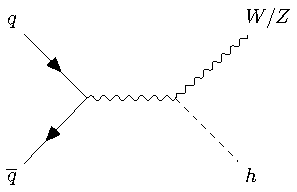
\includegraphics[width=0.4\textwidth]{Images/higgsprod.pdf}
    \caption*{}
    \labfig{higgsprod}
\end{figure}\\
Here it has to be $Z$ when the initial state is neutral, so final state has to be neutral as well, but it could be a $W$ when the initial state is charged, e.g. when we have $u\overline{d}$. At LHC, $\overline{q}$ is a sea quark, i.e. not one of the three valence quarks, it comes from fluctuations of the vacuum of a virtually produced gluon. Associated Higgs production is again less frequent than GGF. Finally, there is another process which uses the coupling with the top:
\begin{figure}[h]
    \centering
    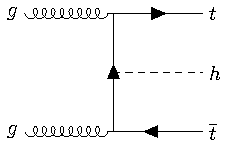
\includegraphics[width=0.4\textwidth]{Images/tth.pdf}
    \caption*{}
    \labfig{tth}
\end{figure}\\
The price to pay is that the top appears also in the final state of other processes so it is possible to have the gluons and then a $t\overline{t}$ pair to which we attach the Higgs. This is $t\overline{t}h$ production which requires a very large $\sqrt{s}$ so its cross section is one of the smallest ones.\\
\marginnote[-2cm]{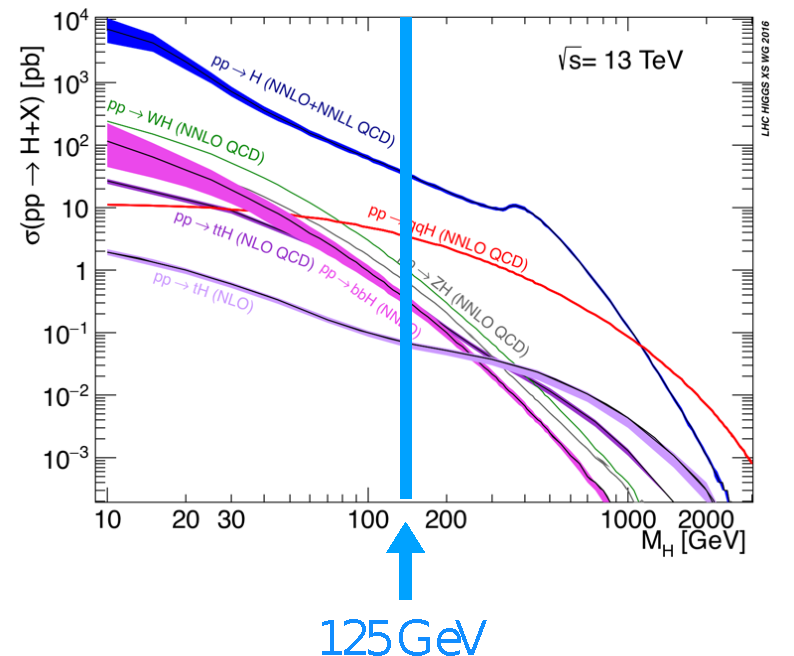
\includegraphics{Images/higgsplot.pdf}\\NNLO is the Next to Next Leading Order and represents some important corrections.}In the plot on the side, a summary of the various cross sections for different values of $m_h$ is shown. The Higgs mass is 125 GeV so we should look at the hierarchy highlighted by the cyan arrow. The total cross section is the sum of all cross sections of these processes and at $\sqrt{s}=13$\,TeV it turns out to be 56 pb. How many Higgs bosons are produced at LHC? In Run 1 there were something like 70k Higgs bosons while in Run 2 almost a million were produced, 900k. Be careful because these are the ones which were produced, they have to be detected and at this point it depends on how the Higgs boson decay.
\subsection{Decay}
The Higgs boson decays into two quarks $H\to q\overline{q}$ but it cannot go into two tops since $m_t=173$\,GeV$>m_h=125$\,GeV, so the largest decay channel into quarks is $b\overline{b}$. This has a branching ratio of something like 60\%. However, detecting $b\overline{b}$ and distinguishing it from all the other quarks that can be produced at LHC is a very difficult challenge. These quarks transform themselves into jets and when the energy decreases they start to form hadrons. This transition is called \textbf{hadronization}, some hadrons can be unstable and they will decay.\\
What are the other possible processes? The Higgs cannot go into two $W$ but one of the two can be virtual and can decay either in $l\overline{\nu}$ or $q\overline{q}$.
\begin{figure}[h]
    \centering
    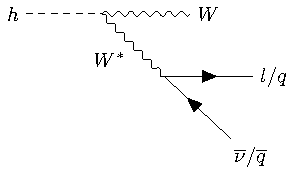
\includegraphics[width=0.45\textwidth]{Images/hd1.pdf}
    \caption*{}
    \labfig{hd1}
\end{figure}\\
The process is then a three-body decay of the Higgs and it has a branching ratio around 30\%. Every time there are quarks things are complicated while with leptons things are easier: the cleanest possibility is when everything is leptonic but then we lose in probability. Another possible decay is the one in which the Higgs goes into two gluons but that is a nightmare because these gluons are submerged by tons of other gluons and quarks but there is a similar process with photons instead of gluons.
\begin{figure}[h]
    \centering
    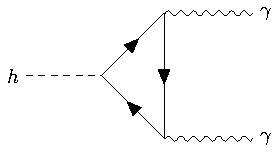
\includegraphics[width=0.45\textwidth]{Images/hphotons.pdf}
    \caption*{}
    \labfig{hphotons}
\end{figure}\\
This is very rare, the branching ratio is 0.2\% but it is very clean because these two photons emerge separately and the invariant mass is 125 GeV. Actually not really clean because there are many many jets which fake photons, so the background we will see is very large and it is not coming from real photons but it comes from jets which eventually leave that energy in the detector and simulate a photon. Photons leave energy in the electromagnetic calorimeter and unfortunately jets do the same, in addition to depositing energy in the hadronic calorimeter. Some of the jets, very rarely, leave a signature which is very similar to the photons. It happens rarely but since we have so many jets there is eventually a significant contribution to the background.\\
One last possible decay process is the one in which the Higgs goes into two $Z$ which then decay each in a pair $ll^+$.
\begin{figure}[h]
    \centering
    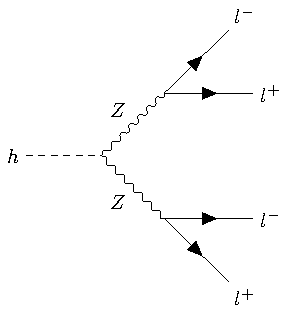
\includegraphics[width=0.45\textwidth]{Images/h4l.pdf}
    \caption*{}
    \labfig{h4l}
\end{figure}\\
Compare it with the situation with the $W$ instead of the $Z$ where there are two charged leptons and two neutrinos and it is not possible to reconstruct the invariant  mass while in this case it is possible to reconstruct both invariant masses and we expect something of 125 GeV. $h\to4l$ and $h\to\gamma\gamma$ were the channels of discovery. A summary of the branching ratios for the different decay channels at $m_h=125$\,GeV is listed in the table below, while in the plot on the side it is possible to see how the branching ratios vary with the Higgs mass.\marginnote[2cm]{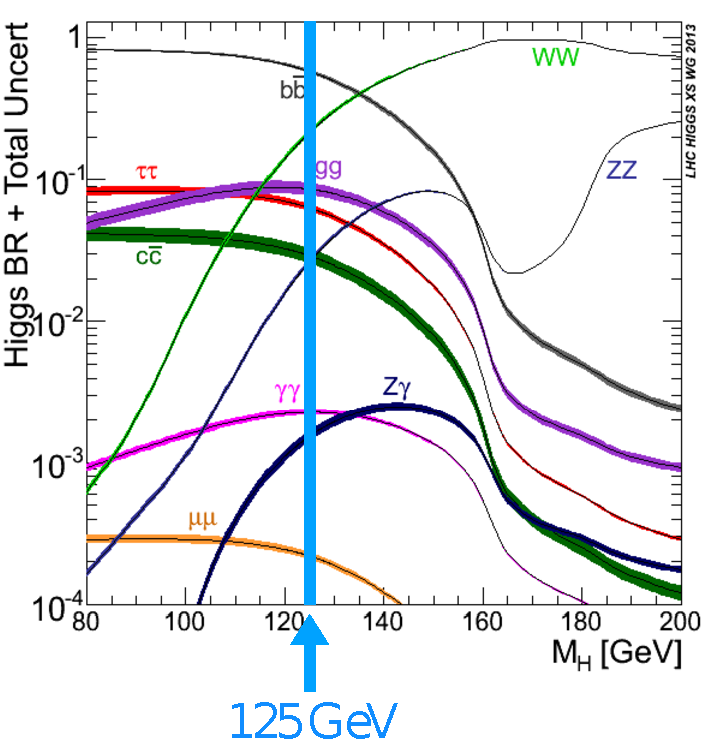
\includegraphics{Images/higgs2.pdf}}
\begin{table}[h]
    \centering
    \begin{tabular}{c|c||c|c}
    \hline
    \rowcolor{gray!45}Process & Branching Ratio & Process & Branching Ratio\\
    \hline
    $b\overline{b}$ & 58\% & gg & 8.2\%\\
    $WW^*$ & 21\% & $Wl\nu$ & 4.6\%\\
    $ZZ^*$ & 2.6\% & $Zll$ & $1.8\times10^{-3}$\\
    $ZZ^*\to4l$ & $1.2\times10^{-4}$ & $\gamma\gamma$ & $2.3\times10^{-3}$\\
    \hline
    \end{tabular}
    \caption{Branching ratios for the different Higgs decay channels ($l=e,\mu$).}
    \labtab{br}
\end{table}\\
Because of its mass, the total Higgs width is very small,  $\Gamma_h=4.1$\,MeV, and the main reason is that the couplings are small.\\ 
One of the predictions of the SM is that the Higgs coupling with two fermions is proportional to $m_\Psi/v$ and with two vectors is proportional to $m_v/v$. There are these proportionality relations which can be tested. The prediction is for a straight line.
\begin{figure}[h]
    \centering
    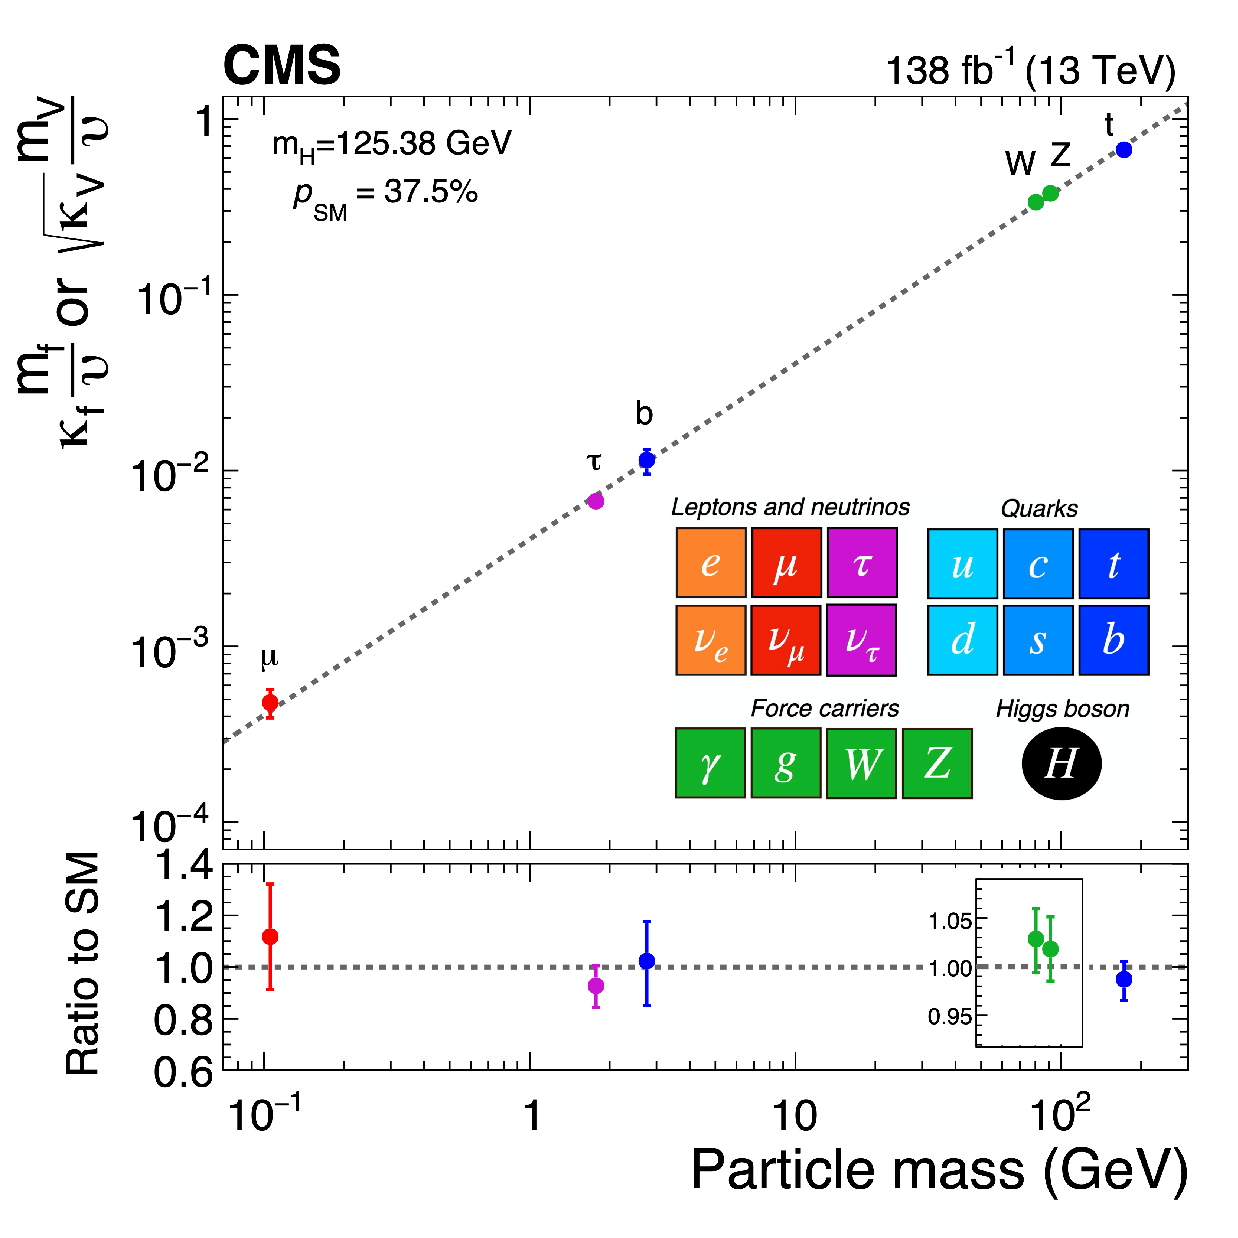
\includegraphics{Images/higgscouplings.pdf}
    \caption*{}
    \labfig{higgscouplings}
\end{figure}\\
Notice how these couplings are so different in strength but they all agree with the SM predictions. It is clear that there is a mechanism which relates the coupling to the mass of the particle. 
\end{document}